\chapter{Introduction}

Since 2010 Deltares is working on a bank erosion module that can be used in combination with D-Flow FM.
The module computes local erosion sensitivity, visualizes the bank movement and gives an estimation of the amount of bank material that is released in the first year and after the equilibrium is reached.
D-FAST Bank Erosion can easily be used as a post processing tool of D-Flow FM-simulations.
Some examples for which D-FAST Bank Erosion can compute bank erosion are:

\begin{itemize}
\item Bank adjustments such as removal of bank protection
\item Applying or removing fore shore protection
\item Changes in shipping type or intensity
\item Changes in currents (e.g. due to construction of side channels)
\end{itemize}

\subsubsection*{Output}
The output of D-FAST Bank Erosion is:

\begin{enumerate}
\item Bank line movement after one year and when the final equilibrium state is reached.
\item Amount of sediment that is released from the banks after one year and when the final equilibrium state is reached.
\end{enumerate}

This output is presented in graphs / figures and written to text files.

\subsubsection*{Input}
The input of D-FAST Bank Erosion is:

\begin{enumerate}
\item D-Flow FM results (NetCDF map-files)
\item Local data: level of bank protection removal, subsoil characteristics, shipping information (quantity, location of fairway)
\end{enumerate}

The layout of this manual is as follows: In this chapter a description is given on how to use D-FAST Bank Erosion (installation, input, output).
The background of D-FAST Bank Erosion is outlined in \autoref{Chp3} and \autoref{Chp4} (partly in Dutch).

\section{Installation}

D-FAST Bank Erosion itself consists of 2 executables called 'BankLines.exe' and BankErosion.exe'.
The first is needed to establish the initial bank lines and the second computes the bank line movement and eroded volume.
Both executables of D-FAST Bank Erosion can be called from the DOS prompt.

To be able to run D-FAST Bank Erosion it is necessary to install MCRinstaller.
The required version of the installer is standard provided with D-FAST Bank Erosion.

By default D-FAST Bank Erosion is looking for the definition file deffile.def in the same directory as the executables.
When the definition file has another name or location, this should be passed when the modules are called.

\section{Scenario plan}

D-FAST Bank Erosion is not calibrated for local bank erosion\footnote{This is almost impossible, due to other uncertainties in bank properties, limited availability of field data of measured bank erosion and the fact that WAQUA computes longer river reaches.
Locally D-FAST Bank Erosion could be calibrated when historical data of bank erosion is available.
However, this does not automatically imply that a few kilometers downstream D-FAST Bank Erosion gives good results with the same settings, because the bank properties can be completely different.}.
Therefore it is strongly advised to use D-FAST Bank Erosion only in a \emph{relative} way.
In this way an image can be formed of

\begin{itemize}
\item at which locations the bank is most sensitive to erosion (by comparing different locations along the river)
\item how sensitive a location is for certain measures (by comparing different scenarios at 1 location)
\end{itemize}

We advise to compute different scenarios and compare between them.
An example is: 1 scenario with a subsoil of sand and 1 scenario with a subsoil of clay.
This means that only the type of subsoil is changed and the other input remains unchanged.

\section{D-Flow FM-computations}

Before D-FAST Bank Erosion can be used, steady state D-Flow FM-computations\footnote{D-Flow FM-models and Baseline schematisations of the Dutch river system can be applied by Helpdeskwater.nl Onderwerpen > Applicaties en modellen > Water en ruimte > Gebiedsschematisaties > Servicedesk > Meldingsformulier} have to be performed for each discharge level.
This first requires a schematisation of the discharge hydrograph in discharge levels and a probability per discharge step.
The discretisation of the discharge hydrograph is not a trivial procedure.
Deltares advises to use at least ten discharge levels.

By default two figures are generated during D-FAST Bank Erosion computation which the user can use to check if the discharge levels are chosen properly.
These are a figure with water levels and a figure with flow velocities.
In both figures the area that is sensitive to erosion is indicated.
Based on these figures it can be decided to include or remove discharge levels from the computation.
For each discharge level an NetCDF map-file (D-Flow FM output file) must be provided.
D-FAST Bank Erosion uses the water levels and flow velocities that are stored in the last time step.
It is important that the D-Flow FM computations are in steady state.
The probability (normalized weighting of the time period) per discharge level is defined by the user in the definition file.

Note: It is of utmost importance that in the NetCDF map-file with the reference (average) discharge (which is used to establish the initial bank lines) the water remains within the main channel during the whole computation.
Practically this means that the simulation has to be started with a low initial water level with no (or as little as possible) water in the flood plains.
When this criterion is not met, strange peaks in the detected bank lines may occur.



An example of discharge levels for the river Meuse in combination with different probabilities for different scenarios (wet/dry/intermediate) is given in \autoref{Tab2.1}.

\begin{table}
\begin{tabular}{p{2cm}p{2cm}p{2cm}p{2cm}p{2cm}}
Dicharge level nr. & Discharge (m3/s) & 1998-2002 (wet) & 2004-2010 (dry) & 2008-2011 (intermediate) \\ \hline
1 & 75 & 0.2932 & 0.1808 & 0.3110 \\
2 & 150 & 0.1918 & 0.2466 & 0.2329 \\
3 & 272 & 0.1918 & 0.2603 & 0.2055 \\
4 & 400 & 0.0411 & 0.0548 & 0.0685 \\
5 & 500 & 0.1507 & 0.1370 & 0.0959 \\
6 & 750 & 0.0548 & 0.0712 & 0.0548 \\
7 & 900 & 0.0329 & 0.0384 & 0.0164 \\
8 & 1100 & 0.0164 & 0.0082 & 0.0055 \\
9 & 1300 & 0.0137 & 0.0014 & 0.0021 \\
10 & 1500 & 0.0041 & 0.0014 & 0.0021 \\
11 & 1700 & 0.0041 & 0.0000 & 0.0021 \\
12 & 1900 & 0.0041 & 0.0000 & 0.0021 \\
13 & 2300 & 0.0014 & 0.0000 & 0.0014 \\ \hline
\end{tabular}
\caption{Probabilities of a discharge level for different scenarios (De Vries, 2012)}
\label{Tab2.1}
\end{table}

\section{Definitionfile <defile.def>}\label{Sec2.4}

The definition file contains input parameters for the executables 'BankLines' en 'BankErosion'.
De executables search for the file 'defile.def' in the same directory as themselves, unless another file or path name is given.
The possible keywords and their description are given in \autoref{Tab2.2}.
The existence, not the order, of the keywords is of importance.

In the table the following abbreviations are used:
\begin{itemize}
\item[M] mandatory
\item[O] optional
\item[E] expert
\end{itemize}

Filenames can be either given with a single filename, or with their (relative) path and they should contain no spaces.
An example of a definition file is given in \autoref{Fig2.1}.

\begin{table}
\begin{tabular}{lllp{5cm}}
Keyword &  & Value & Description \\ \hline
Path & M & pathname & [REMOVED] Pathname of used m-files (unnecessary when using executables) \\
Nbank & M & integer & Number of bank lines, (standard 2 lines) \\
GridFile  & M & filename & Rgf-file for defining grid coordinates \\
RiverKM & M & filename & Textfile with riverkilometres and correspondig xy-coordinates \\
Boundaries  & O & integers & river chainage of the region of interst;  rkm-start:rkm-end, e.g. 81:100 (default: all) \\
NLim & O & integers & [REMOVED] Range of N-values from SDS-file that is considered (default: all), only used when keyword 'Boundaries' is not available. \\
Mlim & O & integers & [REMOVED] Range of M-values from SDS-file that is considered (default: all), only used when keyword 'Boundaries' is not available. \\
Plotting & O & logical & [REMOVED] Plotting results (default: false) \\
SavePlots & O & Logical & [REMOVED] Saving plots (default: true) \\
ClosePlots & O & Logical & [REMOVED] Close plots and close Quickplot when simulation is finished (default: false) \\
Waqview & O & logical & [REMOVED] Generating output for Waqview (default: false) \\ \hline
\end{tabular}
\caption{Keywords in the definition file of D-FAST Bank Erosion}
\label{Tab2.2}
\end{table}

Input BankLines.exe

\begin{tabular}{lllp{5cm}}
Keyword &  & Value & Description \\ \hline
SDS-file & M & filename & [REPLACE BY File] SDS-file for determining representative bank line \\
Line1    & M & filename & Textfile with xy-coordinates of search line 1 \\
LineN    & M & filename & Textfile with xy-coordinaten of search line N \\
BankDir & O & string & Directory for storing bank lines (default: current directory) \\
BankFile & O & filename & Text file(s) in which xy-coordinates of bank lines are stored (default 'bankfile') \\
LocalDir & O & filename & Directory for storing local output (default: 'local') \\
SortLim & E & real & Maximum number of vertices used for sorting (default: 50) \\
Waterdepth & E & real & Water depth used for defining bank line (default 0.0) \\
Dlines & E & nline reals & Distance from pre-defined lines used for determining bank lines (default: 50) \\
Dremove & E & nline reals & Ommiting coordinates that are more than this distance from neighbouring points (default: 5000) \\ \hline
\end{tabular}

Input BankErosion.exe

\begin{tabular}{lllp{5cm}}
Keyword &  & Value & Description \\ \hline
Terosion & M & real & Simulation period  [years] \\
RiverAxis & M & filename & Textfile with xy-coordinates of river axis \\
Fairway  & M & filename & Textfile with xy-coordinates of fairway axis \\
BankType & M & filename/real & Bank strength definition (for each bank line per river-km) \\
Vship  & M & filename/real & Relative velocity of the ships (per river-km) [m/s] \\
Nship  & M & filename/integer & Number of ships per year (per river-km) \\
ShipType & M & filename/integer & Type of ship (per river-km) \\
Draught & M & filename/real & Draught of the ships (per river-km) [m] \\
NLevel & M & integer & Number of discharge levels \\
File1 & M & filename & [REPLACES SDSfile1] NetCDF map-file for computing bank erosion for discharge 1 (only used when 'Nlevel'>1) \\
PDischarge1 & M & real & Probability of discharge 1 (sum of probabilities should be 1) \\
FileN & M & filename & [REPLACES SDSfileN] NetCDF map-file for computing bank erosion for discharge 'Nlevel' (only used when 'Nlevel'>1) \\
PDischargeN & M & real & Probability of discharge 'Nlevel' (sum of probabilities should be 1) \\
RefLevel & O & integer & Reference level: discharge level with SDS-file that is equal to 'SDS-file' (only used when 'Nlevel'>1)  (default: 1) \\
Classes & O & logical & Use classes (true) or critical shear stress (false) in 'BankType' (default: true) \\
ProtectLevel & O & filename & Text file(s) with level of bank protection for each bank line per river-km (default: -1000) \\
Slope & O & filename & Text file(s) with equilibrium slope for each bank line per river-km  (default: 20) \\
OutputDir & O & String & Directory for storing output files \\
BankNew & O & filename & Text file(s) in which new xy-coordinates of bank lines are stored (default 'banknew') \\
BankEq & O & filename & Text file(s) in which xy-coordinates of equilibrium bank lines are stored (default: 'bankeq') \\
EroVol & O & filename & Text file in which eroded volume per river-km is stored (default: 'erovol.evo') \\
OutputInterval & O & real & interval in which the output (eroded volume) is given (default: 1 km) [km] \\
VelFilter & E & logical & Filtering velocity along bank lines (default: true) \\
Revert & E & nline integers & Reverting direction of erosion (default 0) \\
Wave0 & E & real & Distance from fairway axis at which waveheight is zero (default 200 m) \\
Wave1 & E & real & Distance from fairway axis at which reduction of waveheigth to zero starts (default Wave0-50 m) \\
Nwave & E & integer & Number of waves per ship (default 5) \\ \hline
\end{tabular}

\begin{figure}
\begin{verbatim}
    % General input parameters bank erosion module
    NBank          = 2
    GridFile       = inputfiles\maas40m_1.rgf
    RiverKM        = inputfiles\rivkm.xyc
    Boundaries     = 123:128
    WaqView        = true
    Plotting       = true
    %
    % Input parameters bank line detection
    Bankdir        = output\banklines
    SDSfile        = inputfiles\SDS-q272
    Line1          = inputfiles\oeverlijn_links_mod.xyc
    Line2          = inputfiles\oeverlijn_rechts_mod.xyc
    %
    % Input parameters bank erosion module
    OutputDir      = output\bankerosion
    Terosion       = 1
    RiverAxis      = inputfiles\maas_rivieras_mod.xyc
    Fairway        = inputfiles\maas_rivieras_mod.xyc
    Classes        = false
    BankType       = inputfiles\bankstrength_tauc
    Vship          = 5.0
    Nship          = inputfiles\nships_total
    ShipType       = 2
    Draught        = 2.5
    ProtectLevel   = inputfiles\stortsteen
    Slope          = inputfiles\slope
    BankEq         = bankequi
    EroVol         = erovol_standard.evo
    OutputInterval = 0.1
    Revert         = [1,0]
    %
    % Discharge dependent parameters
    NLevel         = 10
    RefLevel       = 3
    SDSfile1       = SDSfiles\SDS-q75
    PDischarge1    =   0.1808
    SDSfile2       = SDSfiles\SDS-q150
    PDischarge2    =   0.2466
    SDSfile3       = SDSfiles\SDS-q272
    PDischarge3    =   0.2603
    SDSfile4       = SDSfiles\SDS-q400
    PDischarge4    =   0.0548
    SDSfile5       = SDSfiles\SDS-q500
    PDischarge5    =   0.1370
    SDSfile6       = SDSfiles\SDS-q750
    PDischarge6    =   0.0712
    SDSfile7       = SDSfiles\SDS-q900
    PDischarge7    =   0.0384
    SDSfile8       = SDSfiles\SDS-q1100
    PDischarge8    =   0.0082
    SDSfile9       = SDSfiles\SDS-q1300
    PDischarge9    =   0.0014
    SDSfile10      = SDSfiles\SDS-q1500
    PDischarge10   =   0.0014
\end{verbatim}
\caption{Example of a definition file for D-FAST Bank Erosion}
\label{Fig2.1}
\end{figure}

\section{Banklines <BankLines.exe>}

determines the representative bank lines within the area of interest (for background information see chapter 3).
The input of Banklines is given through the definition file (deffile.def), see \autoref{Sec2.4}.

When the definition file has the name deffile.def and is located in the same directory as the executable the module can be called as follows:

\begin{Verbatim}
BankLines
\end{Verbatim}

If the definition file has another name and/or is located in another directory the following call should be used:

\begin{Verbatim}
BankLines path\\deffile\_other.txt
\end{Verbatim}

with \command{path} the path to the directory where the definition file is located and \command{deffile\_other.txt} the name of the definition file.

Required input:

\begin{itemize}
\item D-Flow FM-output file (NetCDF map-file) at representative discharge (\command{SDSfile}),
\item Number of bank Lines (\command{Nbank} default two, the left and right bank),
\item For each of the bank lines a file with xy-coordinates of the estimated location of the bank line (\command{Line1}, \command{Line2}, ..., \command{LineN}, with N the number of bank lines)
\item File which links river kilometres to xy-coordinates (\command{RiverKM}),
\end{itemize}


Optional

\begin{itemize}
\item Area of interest in the form of a range of river kilometres or in terms of mn-coordinates (\command{Boundaries} or \command{NLim} and \command{MLim}).
\item Name of the directory to which the output will be written (\command{BankDir})
\end{itemize}

Output:

\begin{itemize}
\item XY-coordinates of the determined bank lines.
\item Plot of the bank lines (optional, \command{Plotting})
\end{itemize}

The computation has ended successfully when the message "BankLines ended successfully!" appears.

An example of the output as is generated with Banklines.exe is shown in \autoref{Fig2.2}.
The water depth is given with colored surfaces (per grid cell), the black lines are the determined bank lines and the river kilometers are displayed on the river axis.

Note: To obtain the best results, the points of the estimated location of the banks given in  \command{Line1}, \command{Line2}, ..., \command{LineN} (obtained for example from the 'oeverlijnen' from Baseline data), should be equally distributed along the bank with a distance that is in the same order of the gridcellsize along the bank.
Large distances between the points will result in inaccurate bank lines.
Adding points inbetween the points will resolve this problem.
Points too close to eachother will result in large computation times, which can be solved by removing unnecessary points.

\begin{figure}
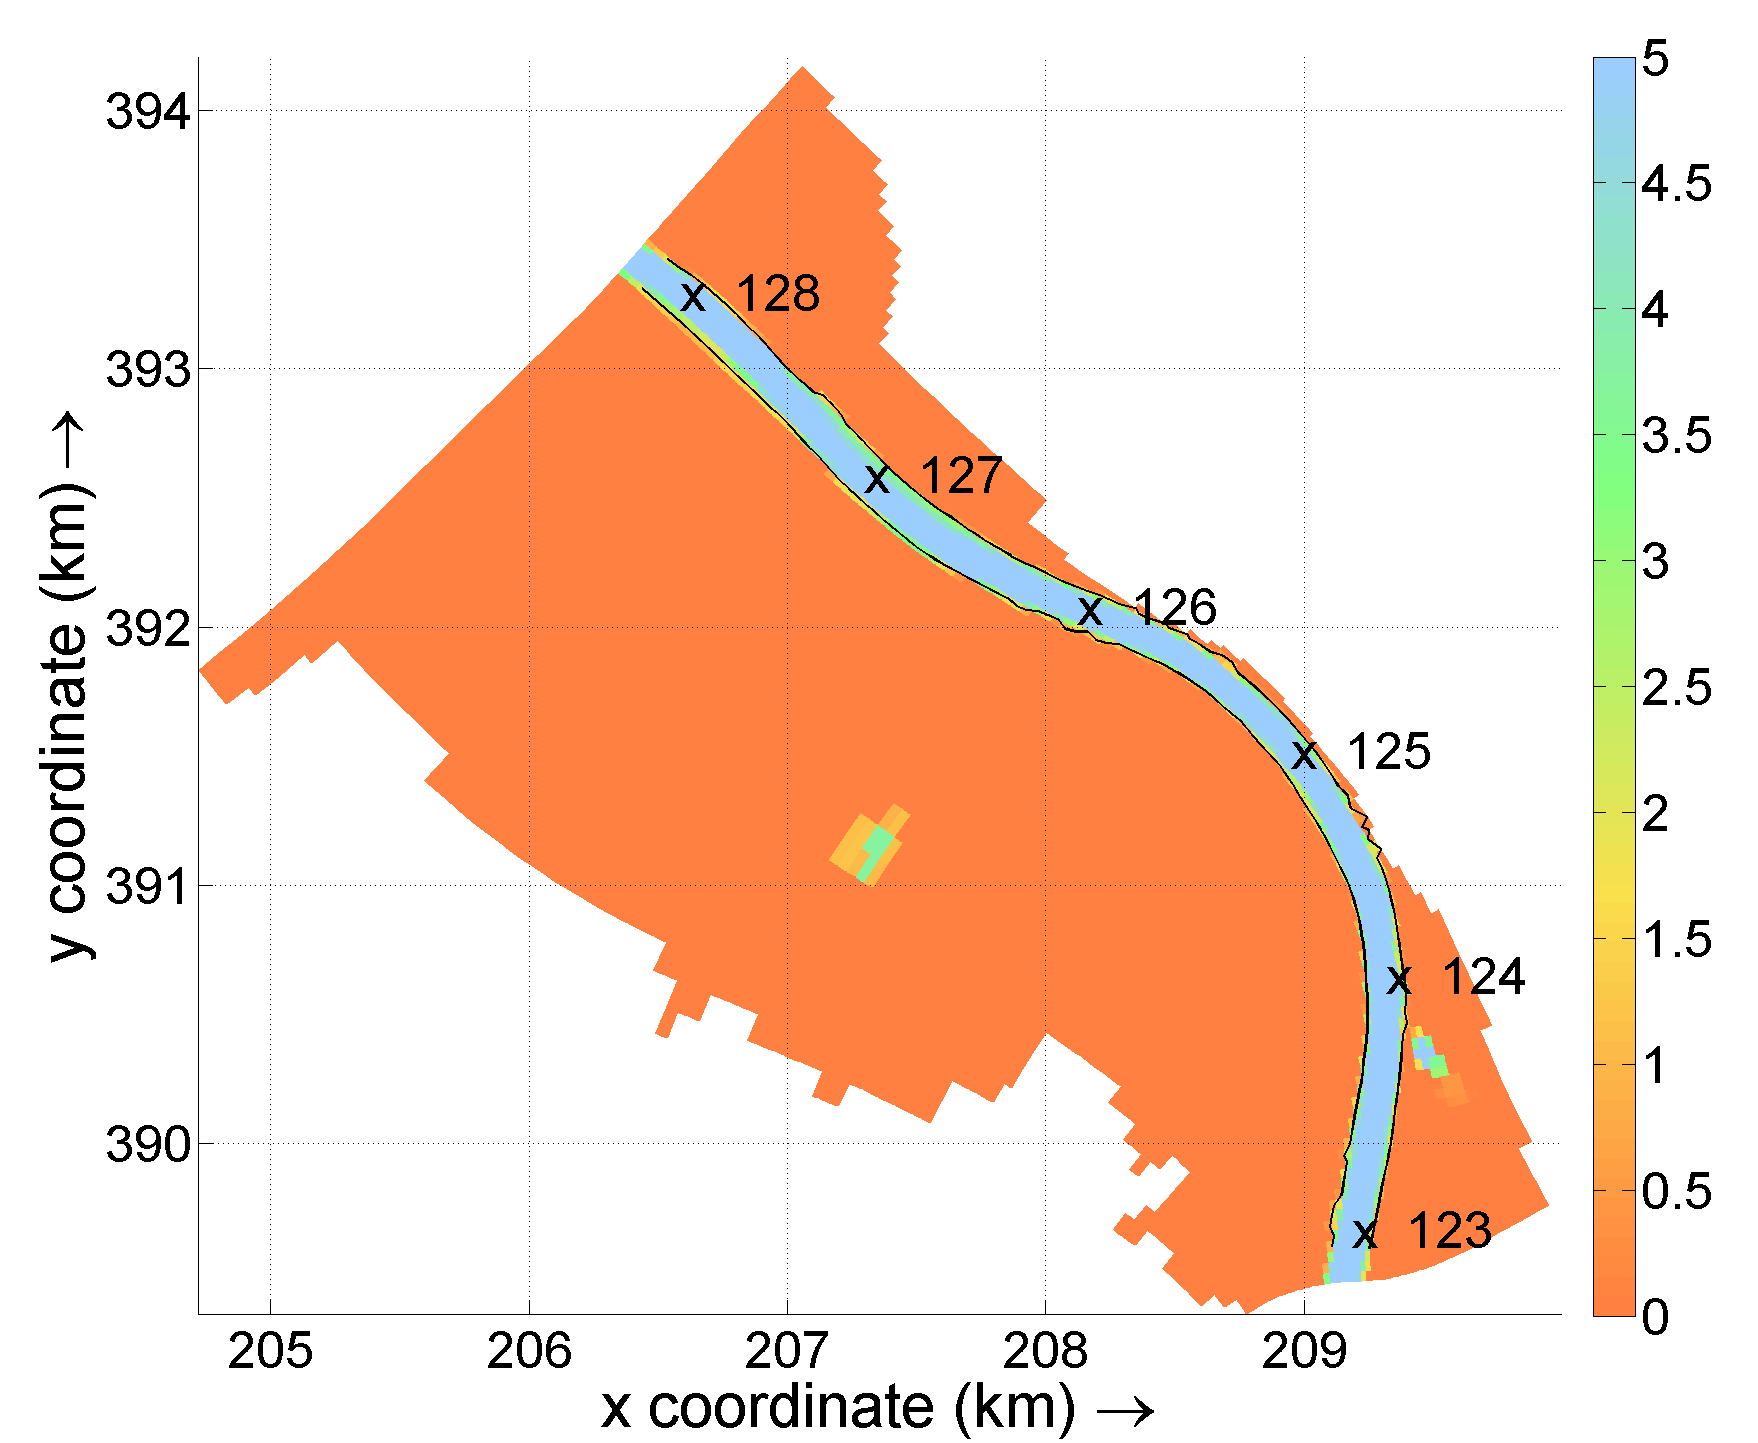
\includegraphics[width=\textwidth]{figures/Fig2-2.png}
\caption{Example of output of BankLines.exe}
\label{Fig2.2}
\end{figure}

\section{BankErosion <BankErosion.exe>}

determines the expected bank erosion within the area of interest (for background information see chapter 4).
The input of BankErosion  is given through the definition file (deffile.def), see \autoref{Sec2.4}.

When the definition file has the name deffile.def and is located in the same directory as the executable the module can be called as follows:

\begin{Verbatim}
BankErosion
\end{Verbatim}

If the definition file has another name and/or is located in another directory the following call should be used:

\begin{Verbatim}
BankErosion path\\deffile\_other.txt
\end{Verbatim}

with \command{path} the path to the directory where the definition file is located and \command{deffile\_other.txt} the name of the definition file.

A clean start can be made with the command:

\begin{Verbatim}
BankErosion deffile.def clean
\end{Verbatim}

This assures that all local files (in the directory \command{LocalDir}), which are specific for a certain reach and discharge levels, are removed.
At the next call of BankLines they are created once again.
The creation of these files can be time consuming, so it is recommended not to clean the files when the reach and/or used SDS-files are not changed.

Required input:

\begin{itemize}
\item The considered simulation time (\command{Terosion}, default 1 year),
\item The number of discharge levels (\command{NLevel}),
\item D-Flow FM-output files (NetCDF map-files) for the different discharge levels and the corresponding probability distribution (\command{File1, File2, ..., FileN} and \command{PDischarge1, PDischarge2, ..., PDischargeN}, with N the number of discharge levels).
When only 1 discharge level is given, the standard NetCDF map-file (\command{SDSfile}) is used,
\item Grid for positioning of results (\command{GridFile}), only needed when \command{WaqView=true},
\item Number of bank Lines (\command{Nbank} default two, the left and right bank),
\item File which links river kilometres to xy-coordinates (\command{RiverKM}),
\item XY-coordinates of the river and fairway axis (\command{RiverAxis}, \command{Fairway}),
\item Information about the strength or type of the soil of the banks (\command{BankType}).
This can be done either in the form of classes (see Tabel 4.1 for values and explanation) or with a critical shear stress (see \autoref{Tab5.1} for examples).
In the first case \command{Classes=true} should be set and in the second case \command{Classes=false} (default).
The bank strength information can be given either with a fixed value for the whole track or in a ASCII-file per river kilometer (first column river-km, second column bank type, see \autoref{Fig2.3}),
\item Shipping information (\command{Vship}, \command{Nship}, \command{ShipType}, \command{Draught}).
This can be done either with a fixed value for the whole track or in a file per river kilometer (first column river-km, second column shipping information: similar to entering bank type, see \autoref{Fig2.3}).
\end{itemize}

Optional
\begin{itemize}
\item ASCII-file with level of bank protection (wrt NAP) for each bank line per river-km.
(First column river-km, second column bank protection level: similar to entering bank type, see \autoref{Fig2.3}).
By default the bank protection level is 1 meter below the water level of the representative discharge,
\item ASCII-file with slope of foreshore (1:n) for each bank line per river-km.
(First column river-km, second column slope parameter n: similar to entering bank type, see \autoref{Fig2.3}).
Default a slope of 1:20 will be used,
\item Name of the directory to which the output will be written (\command{OutputDir}),
\item Name of the file to which the results will be written (\command{BankNew}, \command{BankEq}, \command{EroVol}),
\item Name of the directory to which local files will be written (\command{LocalDir}).
\end{itemize}

Output:

\begin{itemize}
\item Map with waterdepth, initial bank lines, river kilometers and fairway axis (see \autoref{Fig2.4}),
\item Map with erosion sensitivity of the banks based on computed bank retreat (see \autoref{Fig2.5}),
\item The computed erosion volume during the simulation period split up for left and right bank and for each discharge level (see \autoref{Fig2.6}),
\item Total erosion volume based on equilibrium bank line (see \autoref{Fig2.7}),
\item Control figures for water levels of each discharge (see \autoref{Fig2.8} and \autoref{Fig2.9}),
\item Control figures for flow velocity of each discharge (see \autoref{Fig2.10} and \autoref{Fig2.11}),
\item Map with indication of applied bank type (see \autoref{Fig2.12}),
\item Bank retreat at the end of the simulation period and for the equilibrium situation (see \autoref{Fig2.13}),
\item XY-coordinates of the computed bank lines at the end of the simulation period and of the equilibrium bank lines,
\item Files to be able to visualize information in Waqview.
\end{itemize}

The computation has ended successfully when the message "BankErosion ended successfully!" appears.

\begin{figure}
\begin{Verbatim}
  0.0          1
  75.2         3
  90.3         2
  110.0        0
  130.5        4
  153.1        3
  206.9        2
\end{Verbatim}
\caption{Example of input file for bank strength classes per river kilometer: from 0.0 - 75.2 km class 1, from 75.2 - 90.3 km class 3, etc.
When no information is available, the closest value will be used.}
\label{Fig2.3}
\end{figure}

\begin{figure}
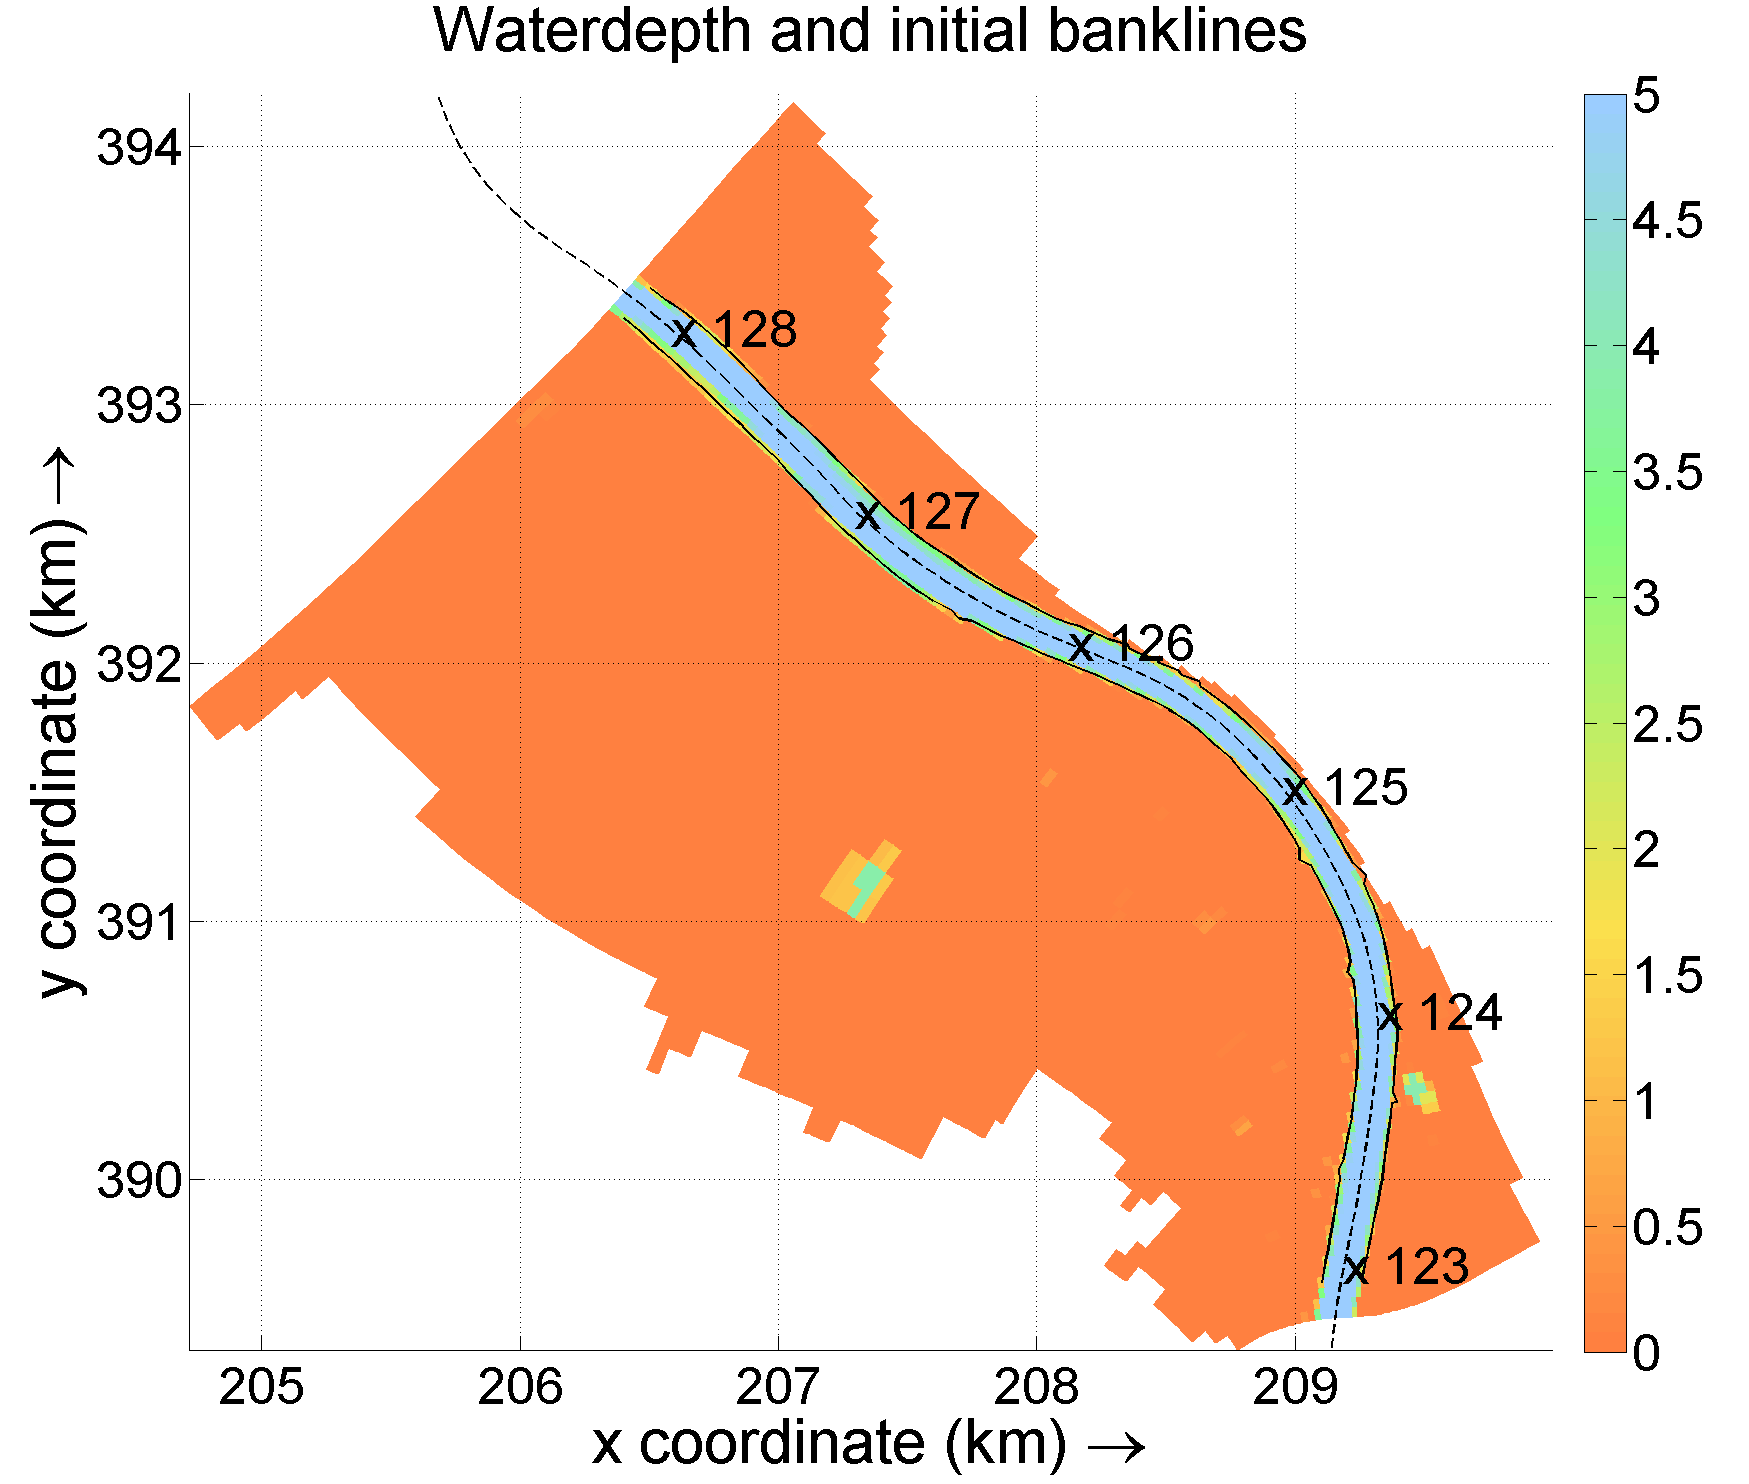
\includegraphics[width=\textwidth]{figures/Fig2-4.png}
\caption{Waterdepth, initial bank lines, river kilometers and fairway axis}
\label{Fig2.4}
\end{figure}

\begin{figure}
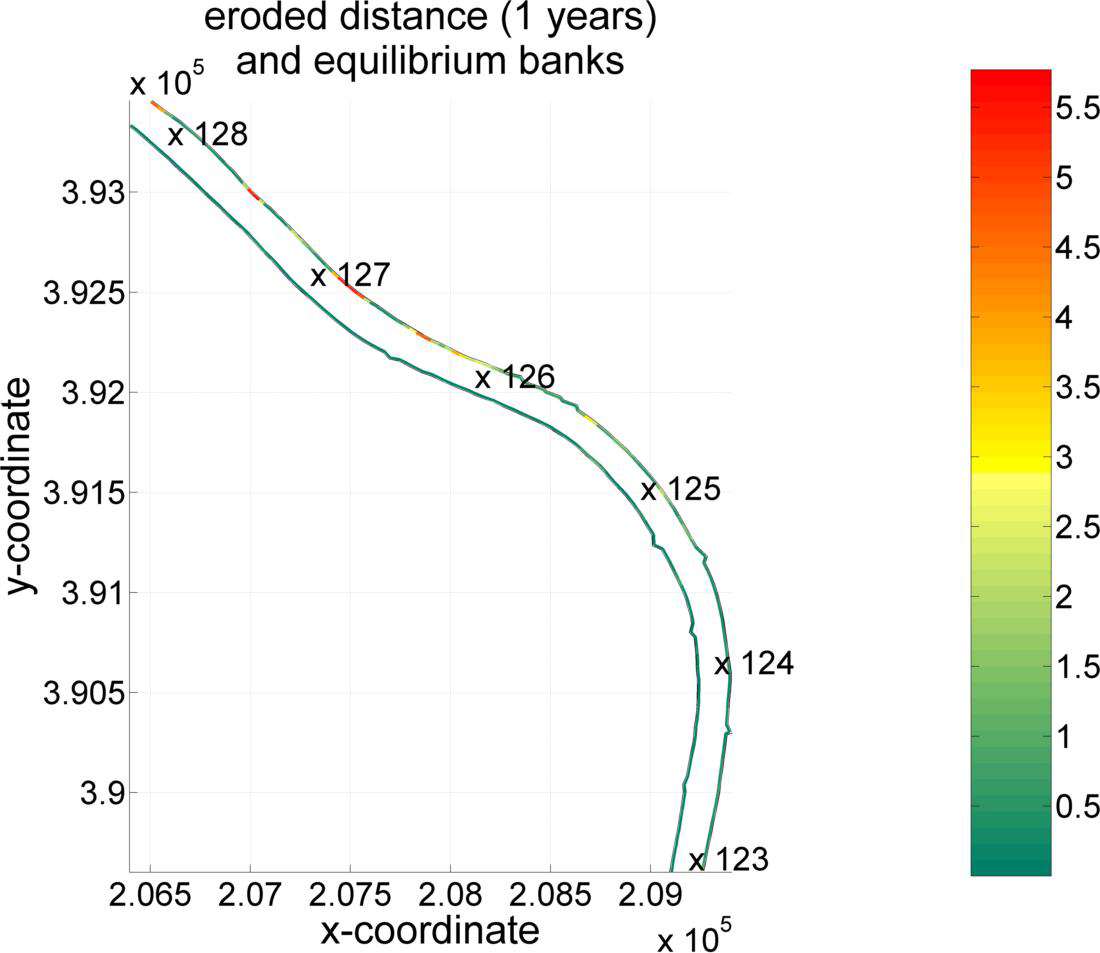
\includegraphics[width=\textwidth]{figures/Fig2-5.png}
\caption{Erosion sensitivity}
\label{Fig2.5}
\end{figure}

\begin{figure}
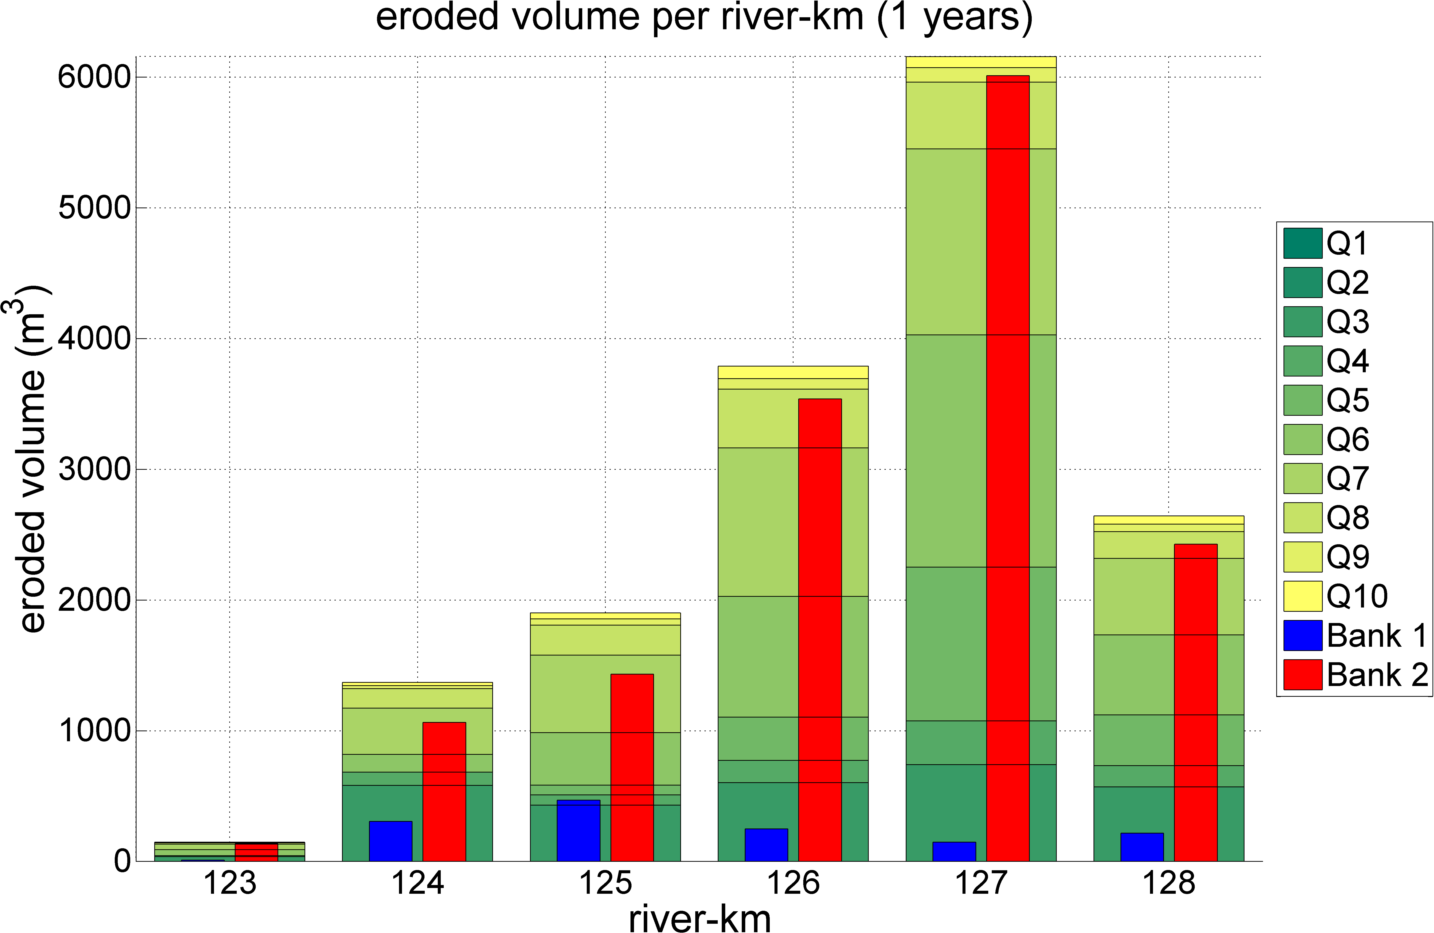
\includegraphics[width=\textwidth]{figures/Fig2-6.png}
\caption{Eroded volume at the end of the simulation period}
\label{Fig2.6}
\end{figure}

\begin{figure}
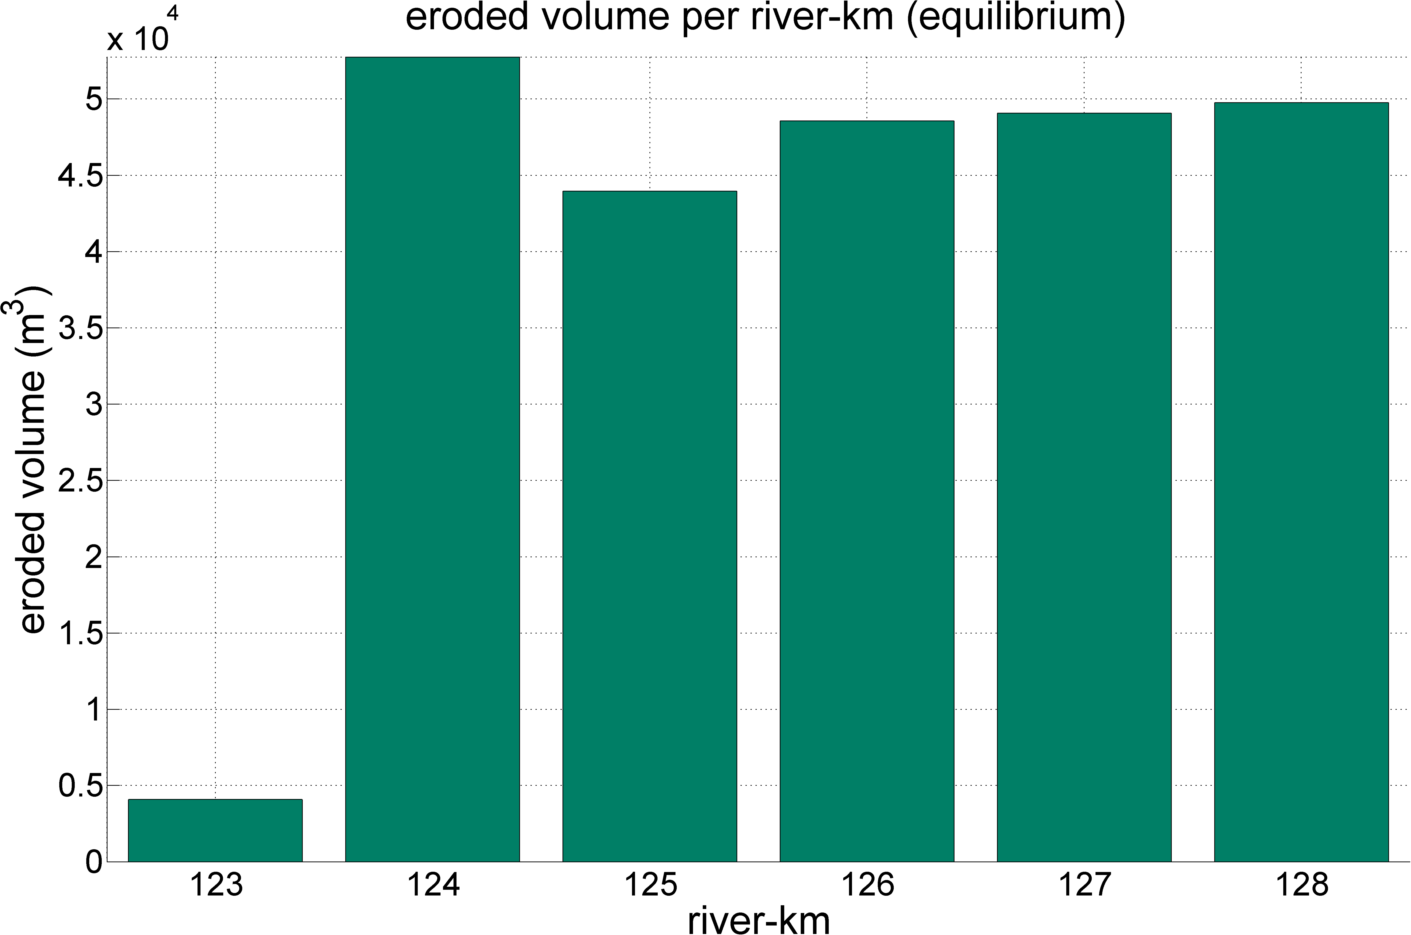
\includegraphics[width=\textwidth]{figures/Fig2-7.png}
\caption{Total erosion volume based on equilibrium bank line}
\label{Fig2.7}
\end{figure}

\begin{figure}
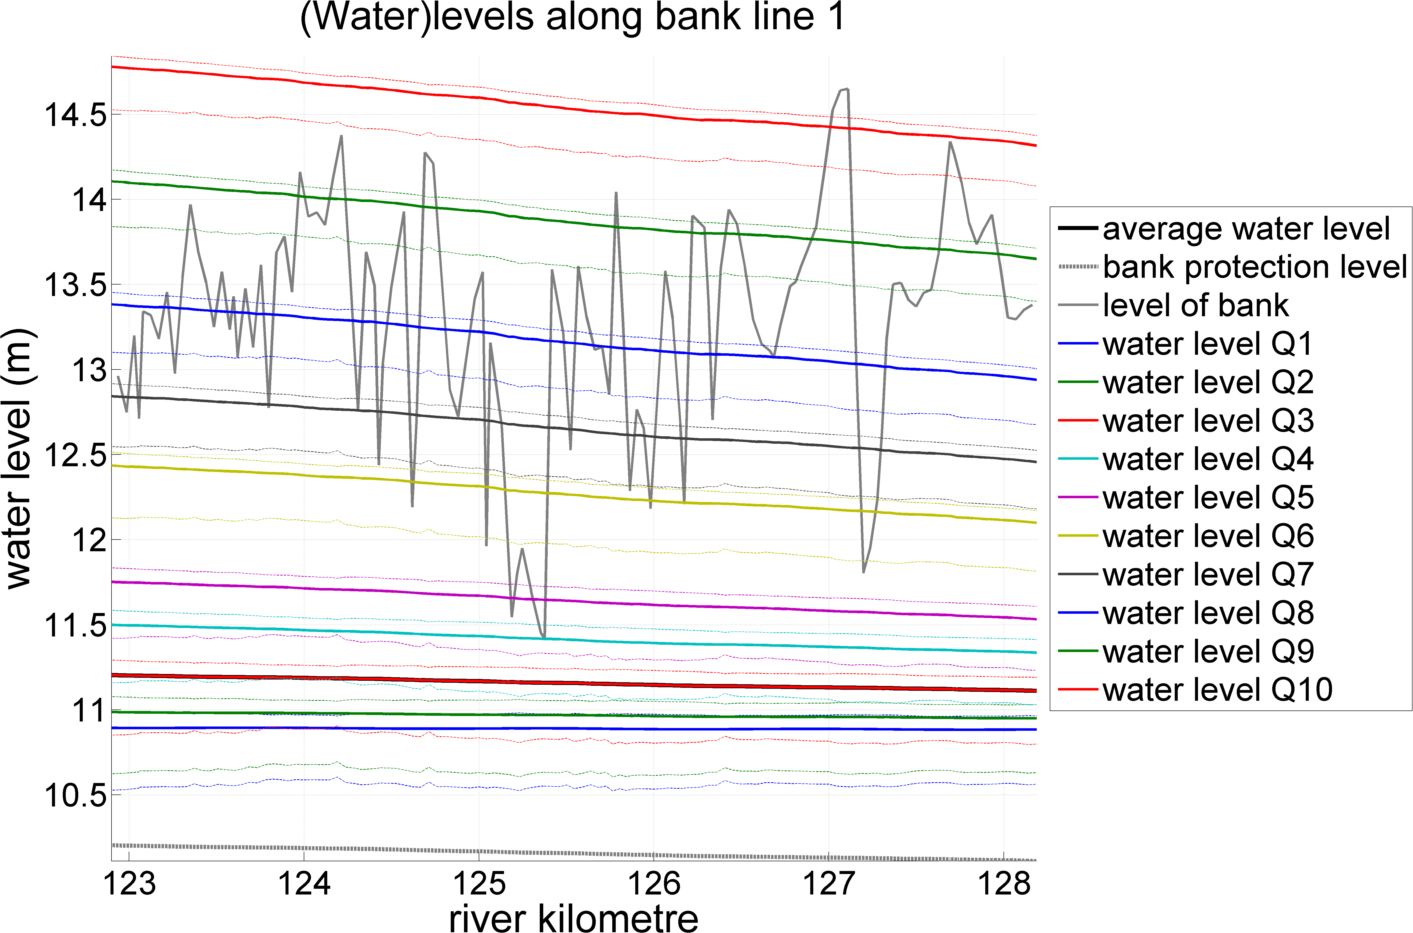
\includegraphics[width=\textwidth]{figures/Fig2-8.png}
\caption{Control figure for water levels of each discharge (bank line 1)}
\label{Fig2.8}
\end{figure}

\begin{figure}
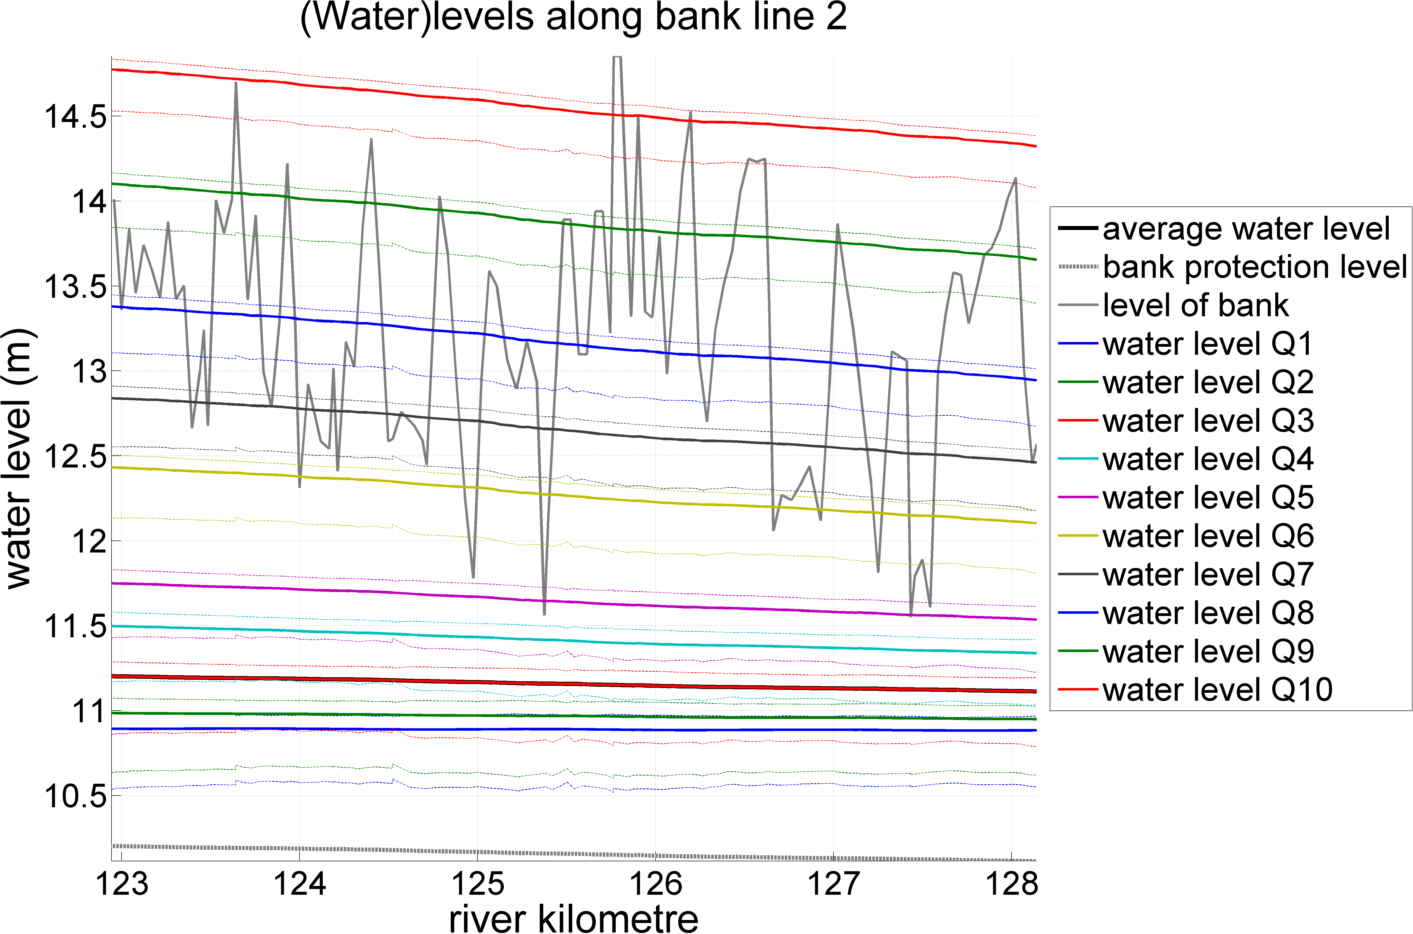
\includegraphics[width=\textwidth]{figures/Fig2-9.png}
\caption{Control figure for water levels of each discharge (bank line 2)}
\label{Fig2.9}
\end{figure}

\begin{figure}
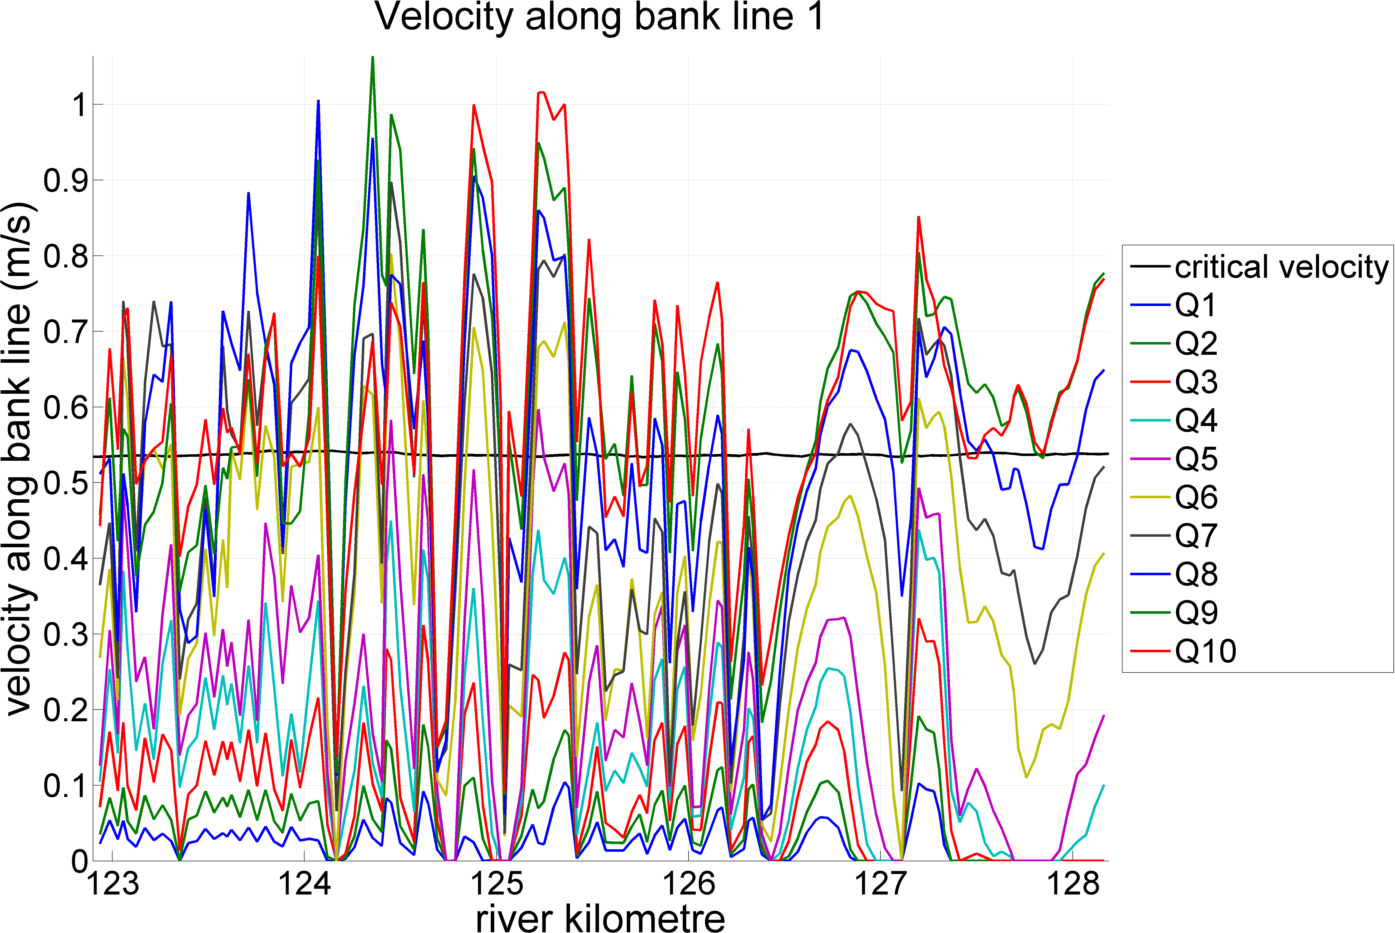
\includegraphics[width=\textwidth]{figures/Fig2-10.png}
\caption{No caption}
\label{Fig2.10}
\end{figure}

\begin{figure}
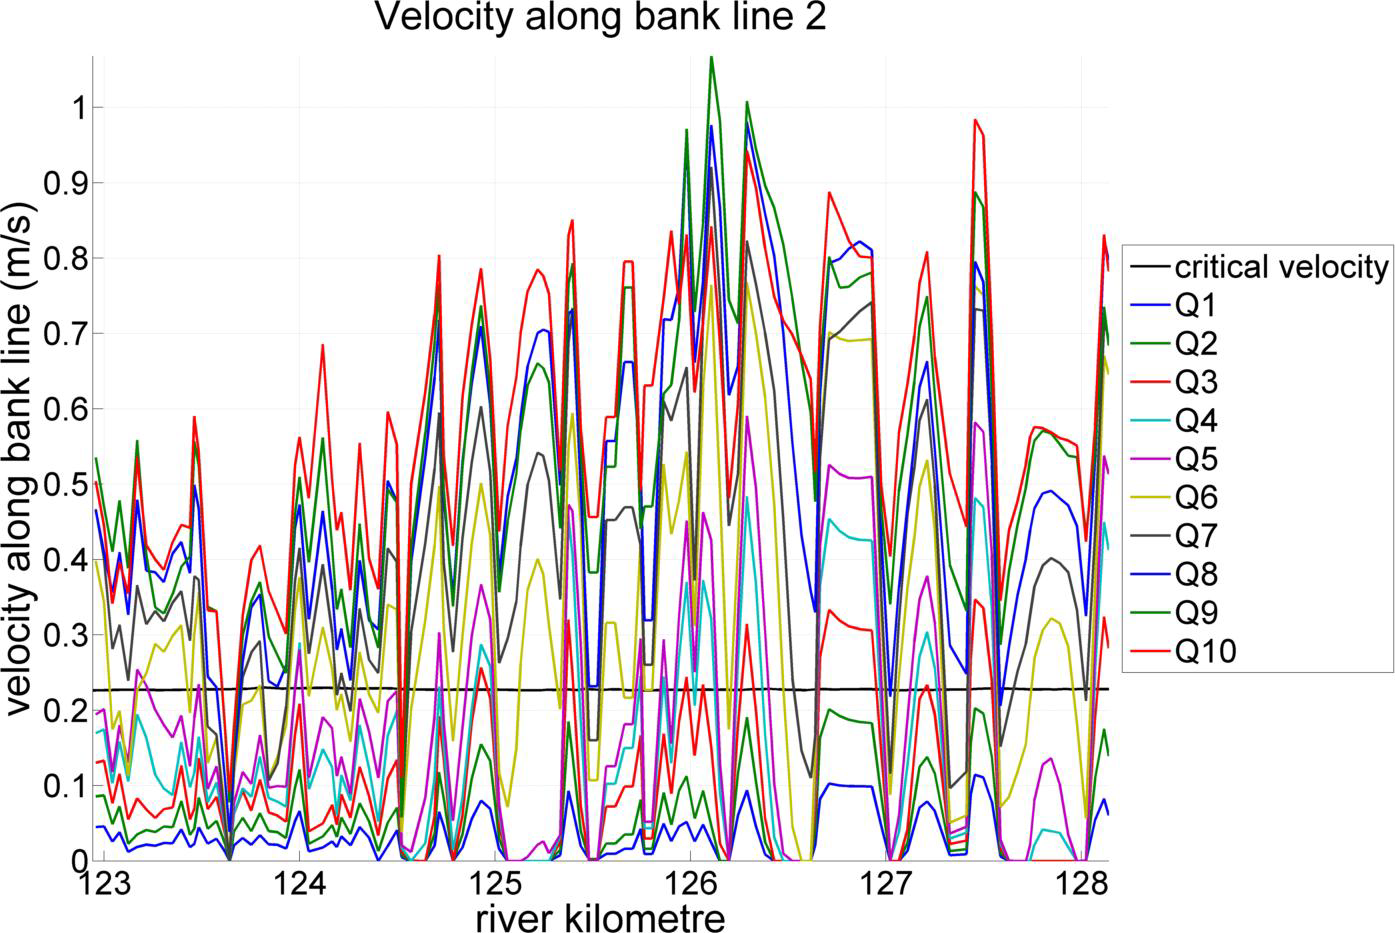
\includegraphics[width=\textwidth]{figures/Fig2-11.png}
\caption{No caption}
\label{Fig2.11}
\end{figure}

\begin{figure}
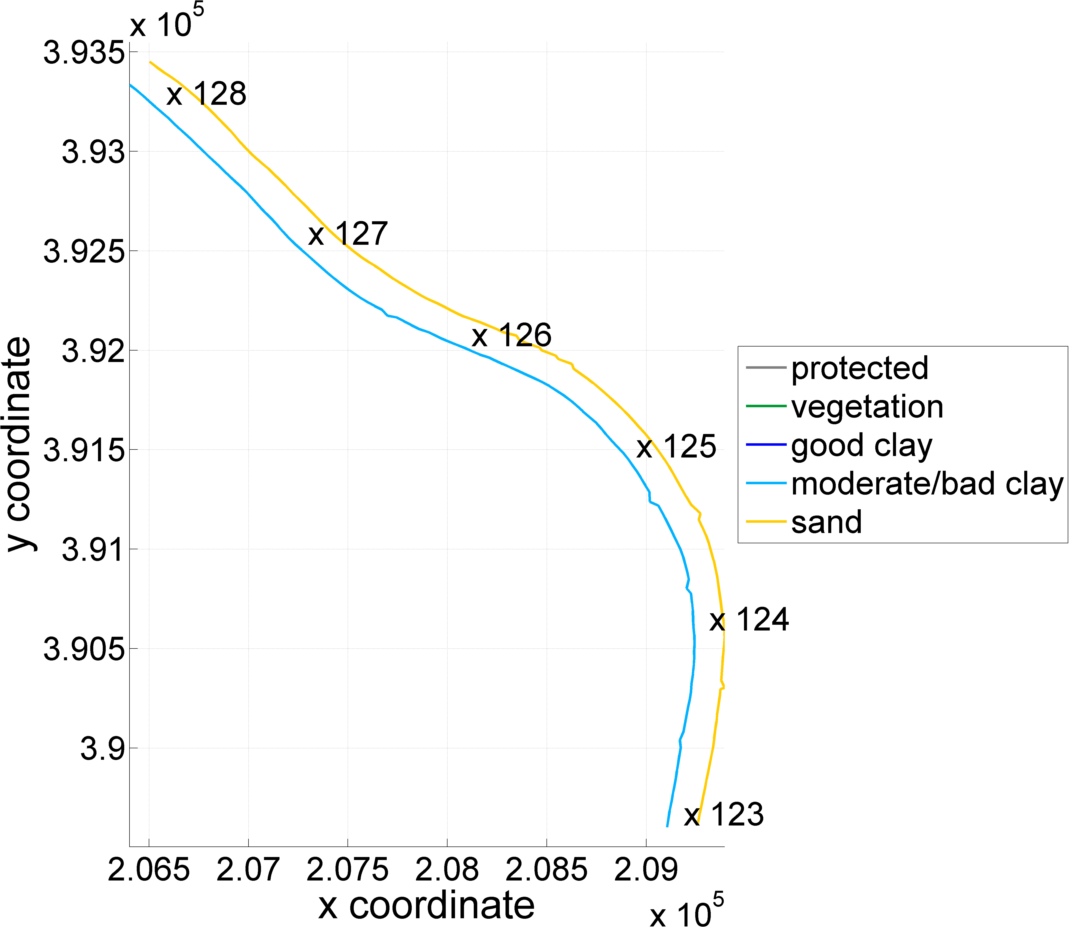
\includegraphics[width=\textwidth]{figures/Fig2-12.png}
\caption{Map with indication of applied bank type}
\label{Fig2.12}
\end{figure}

\begin{figure}
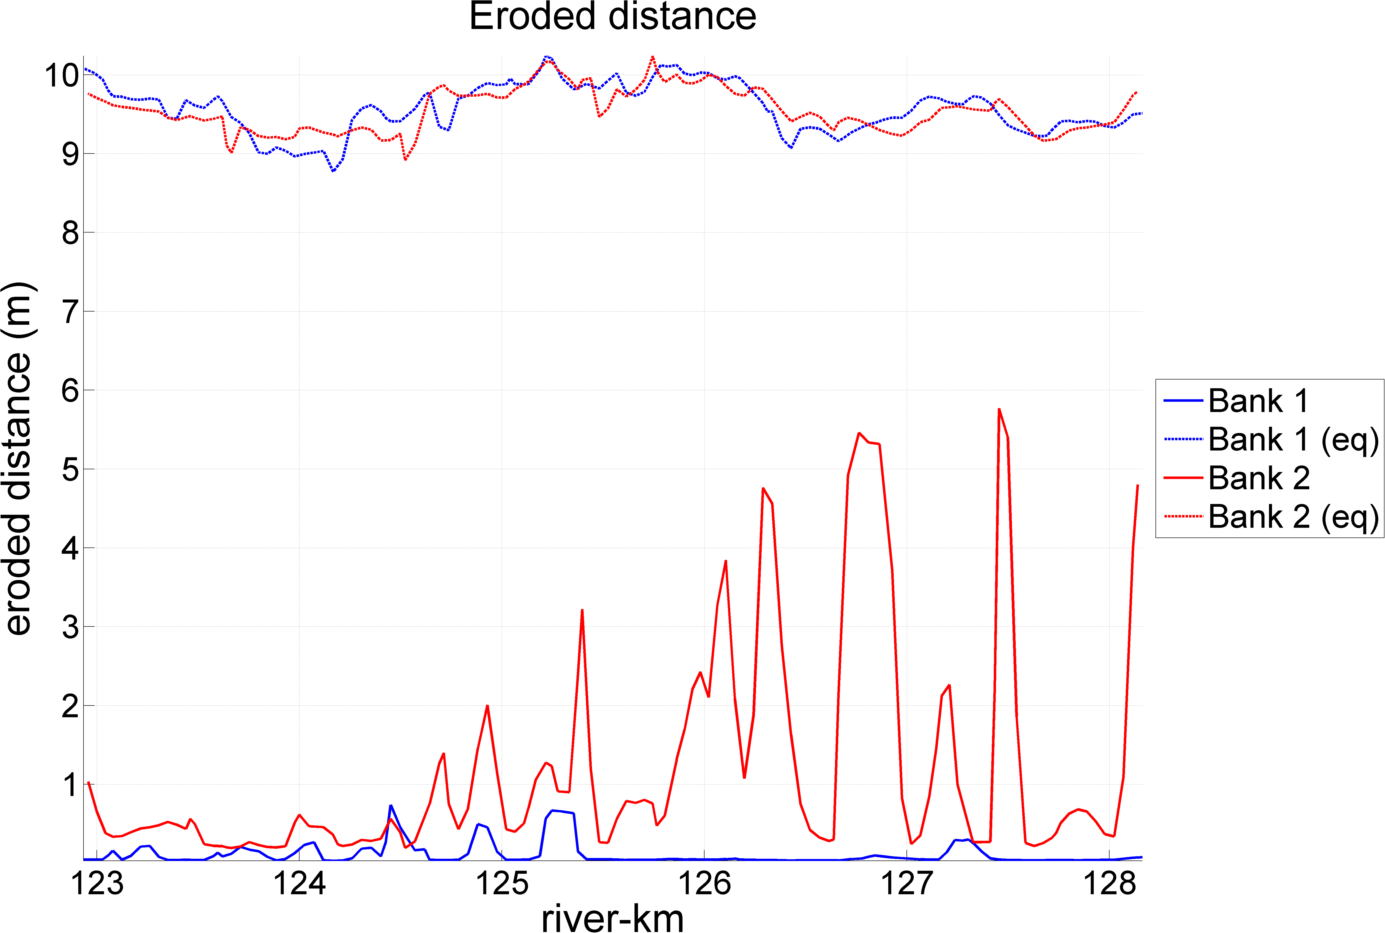
\includegraphics[width=\textwidth]{figures/Fig2-13.png}
\caption{Bank retreat at the end of the simulation period and for the equilibrium situation}
\label{Fig2.13}
\end{figure}
